\chapter{Algoritmy řešící [n,k]-Mastermind}

\section{Kategorie algoritmů}
% přidat definici algoritmu, který řeší mastermind - vytvoří posloupnost kódů, která končí tajným kódem s nejlepším ohodnocením. 
Algoritmy řešící hru Mastermind lze rozdělit do dvou kategorií, \textbf{deterministické} a \textbf{nedeterministické}. Deterministický algoritmus pro dva shodné stavy volí další krok vždy jednoznačně. Nemůže se tedy stát, že by deterministický algoritmus pro dva stejné vstupy vrátil odlišné výsledky. Nedeterministické algoritmy naproti tomu mohou mít v každém stavu na výběr z více následujících kroků. Volit mohou například podle nějakého pravděpodobnostního rozdělení. Není tedy zaručeno, že pro stejný vstup vrátí vždy identický výsledek.

Hlavní předností deterministických algoritmů je záruka výsledku. Na druhou stranu ale tyto typy algoritmů mohou mít velikou časovou složitost, protože jsou často založeny na procházení všech možností pokračování. To se snaží řešit nedeterministické algoritmy, které hledají rovnováhu mezi časovou složitostí a dobrými výsledky. 

V této práci budeme zkoumat pouze deterministické algoritmy. 

% šlo by zmínit výhody a nevýhody (ne)deterministických algoritmů
% Popsat algoritmy, které hrají pouze kandidáty????


\section{Deterministické algoritmy}
% mozna napsat pozdeji ... Všechny deterministické algoritmy, které budeme srovnávat ...

\subsubsection{stav hry}
V každém kroku algoritmů vycházíme z určitého stavu hry, pro který daná metoda vybírá další pokus. Stav je posloupnost pokusů s ohodnocením a jsou to přesně ty informace, které má hráč [n,k]-Mastermindu k dispozici.

\begin{definice}[Stav]\label{stav}
   Nechť $u_i, i\in \{1,2,\dots m\}$ jsou kódy a $r_i = (b_i,w_i)$ jsou ohodnocení. Stav definujeme jako posloupnost $((u_1, r_1), \dots, (u_m, r_m))$. Počáteční stav definujeme jako prázdnou posloupnost.
\end{definice}

Pro každý stav lze nalézt množinu kódů, které by podle dostupných informací mohly být tajným kódem. Jde o ty kódy, které mají s kódy ve stavu stejné ohodnocení jako příslušná ohodnocení ve stavu. 

\begin{definice}[kandidát]\label{kandidat}
  Nechť $P = \left((u_1, r_1), (u_2,r_2), \dots, (u_j,r_j)\right), u_i \in H_{n,k}, r_i \in \N _0 \times \N _0$ je stav. Řekneme, že kód $u \in H_{n,k}$ je kandidát stavu $P$, pokud $s(u,u_i) = r_i \hspace{5px} \forall i \in \{1, \dots j\}$. Pro počáteční stav definujeme množinu kandidátů jako celý prostor kódů $H_{n,k}$.

  % Dále definujeme funkci $J$, která stavu přiřadí jeho množinu kandidátů.
  % \begin{align*}
  %     J \colon (H_{n,k} \times S)^+ &\to \mathbb{R} \\
  %       \left((u_1, r_1), (u_2,r_2), \dots, (u_j,r_j)\right) &\mapsto \{u \in H_{n,k} \mid s(u,u_i) = r_i \hspace{5px} \forall i \in \{1, \dots j\} \} 
  % \end{align*}
\end{definice}
Množina kandidátů dává intuici za tím, jak blízko jsme uhádnutí tajného kódu. V případě, že množina kandidátů je jednoprvková, tak nám je znám tajný kód. Pokud je množina kandidátů veliká, nejspíš ještě budeme k rozlišení tajného kódu potřebovat více pokusů.


Možný průběh hry popíšeme jako kořenový strom, kde vrcholy odpovídají stavům hry. Hrany znázorňují pokusy s ohodnocením, které hru posouvají do dalších stavů. 

\begin{definice}[Strom \text{[n,k]-Mastermindu}]
  Strom \text{[n,k]-Mastermindu} definujeme jako orientovaný graf na množině stavů. Kořenem je počáteční stav. Ze stavu $A = \left((u_1, r_1), (u_2,r_2), \dots, (u_j,r_j)\right)$ do stavu $B = \left((w_1, s_1), (w_2,s_2), \dots, (w_l,s_l)\right)$ vede hrana právě tehdy, když $l = j+1$ a $\forall i \in \{1,2,\dots, j\} \colon (u_i, r_i) = (w_i, s_i)$. Tuto hranu značíme $(w_l, s_l)$. 
\end{definice}

Obrázek \ref{fig22prvnitah} zobrazuje počáteční stav a všechny stavy, do kterých se lze dostat po prvním pokusu. 


\begin{figure}[h!]
    \centering
    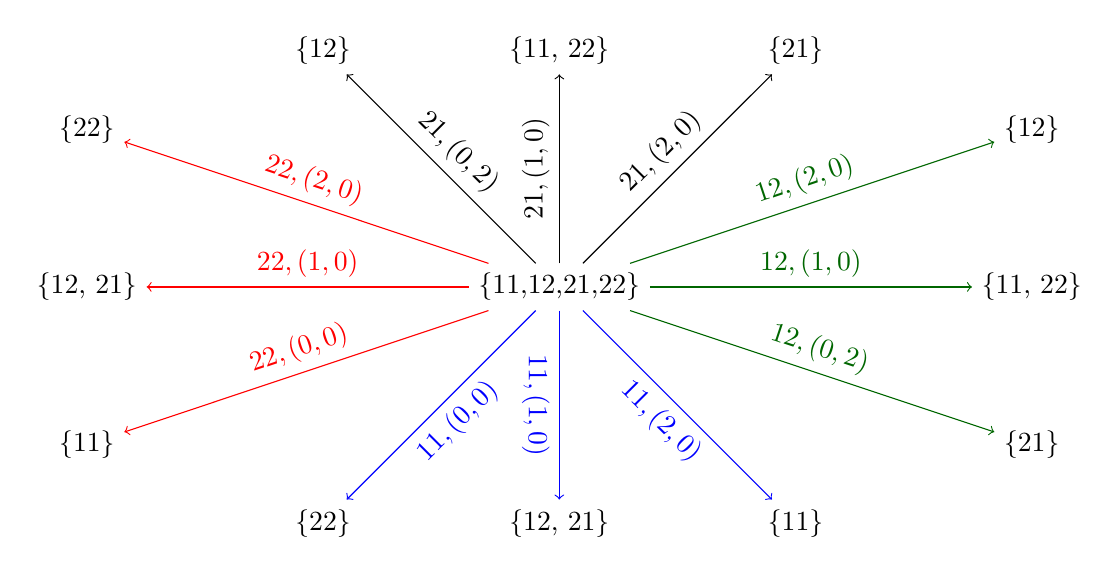
\begin{tikzpicture}
    \node (1) at (0,0) {\{11,12,21,22\}};
    
    \node (2) at (-3,-3) {\{22\}};
    \draw[->,blue] (1) -- (2) node[pos=0.5, below, sloped] {$11,(0,0)$};
    \node (3) at (0,-3) {\{12, 21\}};
    \draw[->,blue] (1) -- (3) node[pos=0.5, below, sloped] {$11,(1,0)$};
    \node (4) at (3,-3) {\{11\}};
    \draw[->,blue] (1) -- (4) node[pos=0.5, below, sloped] {$11,(2,0)$};
    
    \node (5) at (6,-2) {\{21\}};
    \draw[->,black!60!green] (1) -- (5) node[pos=0.5, above, sloped] {$12,(0,2)$};
    \node (6) at (6,0) {\{11, 22\}};
    \draw[->,black!60!green] (1) -- (6) node[pos=0.5, above, sloped] {$12,(1,0)$};
    \node (7) at (6,2) {\{12\}};
    \draw[->,black!60!green] (1) -- (7) node[pos=0.5, above, sloped] {$12,(2,0)$};

    \node (8) at (-3,3) {\{12\}};
    \draw[->] (1) -- (8) node[pos=0.5, above, sloped] {$21,(0,2)$};
    \node (9) at (0,3) {\{11, 22\}};
    \draw[->] (1) -- (9) node[pos=0.5, above, sloped] {$21,(1,0)$};
    \node (10) at (3,3) {\{21\}};
    \draw[->] (1) -- (10) node[pos=0.5, above, sloped] {$21,(2,0)$};

    \node (11) at (-6,-2) {\{11\}};
    \draw[->,red] (1) -- (11) node[pos=0.5, above, sloped] {$22,(0,0)$};
    \node (12) at (-6,0) {\{12, 21\}};
    \draw[->,red] (1) -- (12) node[pos=0.5, above, sloped] {$22,(1,0)$};
    \node (13) at (-6,2) {\{22\}};
    \draw[->,red] (1) -- (13) node[pos=0.5, above, sloped] {$22,(2,0)$};


    \end{tikzpicture}
    \caption{Graf všech potomků $H_{2,2}$}
    \label{fig22prvnitah}
\end{figure}

Stavy, do kterých ze stavu $A$ vede nějaká hrana nazýváme potomky $A$.

\begin{definice}[Potomek stavu a množiny]\label{potomek}
  % Uvažujme [n,k]-Mastermind s nějakým tajným kódem $v\in H_{n,k}$. 
  % Nechť $S$ je množina všech ohodnocení v $H_{n,k}$. Nechť $A = \left((u_1, r_1), \dots, (u_j,r_j)\right)$ je stav, $u \in H_{n,k}$ je kód a $r \in S$ ohodnocení. Potomka stavu $A$ vzhledem ke kódu $u$ a ohodnocení $r$ definujeme jako stav $A_{u,r} = (\left((u_1, r_1), \dots, (u_j,r_j) ,(u,r)\right)$. 
  
  Potomek stavu $A$ vzhledem ke kódu $u$ a ohodnocení $r$ je stav, do kterého vede ze stavu $A$ hrana $(u,r)$ a značíme ho $A_{u,r}$. 
  
  Nechť $K \subset H_{n,k}$ je množina kódů, potom potomka množiny $K$ vzhledem ke kódu $u$ a ohodnocení $r$ definujeme jako množinu
  \[K_{u,r} = \{w \in K \mid s(u,w) = r\}.\] 
\end{definice}

\begin{pozn}
    Používáme stejné názvosloví pro dva různé objekty. Jejich význam je ale obdobný. Označíme-li $K$ množina kandidátů stavu $A$, tak množina kandidátů stavu $A_{u,r}$ je právě právě $K_{u,r}$. Množina $K_{u,r}$ ale může odpovídat potomkům stavu vzhledem k různým kódům. 
    % Množina kandidátů neurčuje jednoznačně stav (například prohozením prvků stavu bychom došli do stejné množiny kandidátů). Naopak stav jednoznačně určuje množinu kandidátů. 
    % V případě, kdy je určen kód $u$ pro nějaký stav $A$, tak potom množina kandidátů jednoznačně určuje 
    % Platí, že množina kandidátů potomka stavu je potomek množiny. Potomek množiny ale může odpovídat více stavům. 
    Potomkem $K$, vzhledem ke kódu $u$ nazýváme množinu $K_{u,r}$ pro nějaké $r \in S$. Potomkem $K$ nazýváme množinu $K_{u,r}$ pro nějaké $u\in H_{n,k}$ a $r \in S$. Obdobně nazýváme potomky stavu. 
\end{pozn}

\begin{lemma}[Vztah potomků]
    Nechť $S$ je množina všech ohodnocení kódů v $H_{n,k}$. Pro každou množinu $K \subset H_{n,k}$ a kód $u \in H_{n,k}$ platí
    \[K = \dot\bigcup_{r\in S} K_{u,r}\]
\end{lemma}
\begin{dukaz}
    Dokážeme obě inkluze. Z definice $K_{u,r}$ platí $\dot\bigcup_{r\in S} K_{u,r} \subset K$. Nechť $u \in H_{n,k}$. Potom pro každý kód $w \in K$ platí, že $w \in K_{u, s(u,w)}$ a tedy $K \subset \dot\bigcup_{r\in S} K_{u,r}$. Zároveň žádný kód $w \in K$ nemůže mít s kódem $u$ dvě různá ohodnocení, a tedy sjednocení je disjunktní. 
\end{dukaz}

% \begin{pozn}
%     Všimněme si, že $K_{u,r} \subset K \hspace{3px}\forall u\in H_{n,k} \hspace{3px}\forall r\in S$. Navíc pro každou množinu $K \subset H_{n,k}$ a kód $u \in H_{n,k}$ platí
%     \[K = \dot\bigcup_{r\in S} K_{u,r}\]
%     protože pro každý kód $w \in K$ platí, že $w \in K_{u, s(u,w)}$.
%     %, tedy že $w$ náleží do potomka $K$ vzhledem ke kódu $u$ a ohodnocení $s(u,w)$. 
% \end{pozn}




\begin{definice}[Prázdný a konečný stav]\label{kandidat}
  Nechť $P = \left((u_1, r_1), (u_2,r_2), \dots, (u_j,r_j)\right), u_i \in H_{n,k}, r_i \in \N _0 \times \N _0$ je stav. Řekneme, že $P$ je prázdný, pokud je množina kandidátů tohoto stavu prázdná. 

  Řekneme, že stav $P$ je konečný, pokud je neprázdný a poslední člen je roven $(u,(n,0))$ pro nějaký kód $u$.
\end{definice}

Prázdný stav nemůže odpovídat průběhu hry Mastermind, protože v tu chvíli žádný kód nemůže být tajným kódem. V reálné hře by ho šlo dosáhnout pouze při chybě v ohodnocení pokusu. Konečný stav odpovídá konci hry, kdy se pokus shoduje s tajným kódem. Množina jeho kandidátů v tu chvíli obsahuje právě tajný kód. 

\subsubsection{Strom algoritmu}
Průběh [n,k]-Mastermindu s nějakým tajným kódem $v$ lze sledovat ve stromu [n,k]-Mastermindu. Nechť $A$ je stav a hráč zvolí další pokus $u$. Touto volbou hráč vybral část potomků, do kterých se stav hry může dostat. Jsou to právě potomci stavu $A$ vzhledem ke kódu $u$. Zadavatel ohodnotí kód $u$ vzhledem ke kódu $v$ ohodnocením $r$. Ohodnocením určí, který stav z potomků $A$ vzhledem ke kódu $u$ bude následovat. Hráč tedy může vybrat jako následující pokus ten, který bude mít nejvhodnější vrstvu potomků vzhledem ke stavu $A$ (například podle množin kandidátů potomků). Z těchto potomků ale neví, do kterého se hra dostane, protože nezná ohodnocení s tajným kódem. 

Předpokládejme, že máme nějaký algoritmus výběru dalšího tahu a pro každý dosažitelný stav $A$ [n,k]-Mastermindu s libovolným kódem $v$ známe následující zahraný kód $u$. Potom lze sestavit takzvaný strom algoritmu, který zobrazuje pro stav $A$ potomky vzhledem k zahranému kódu $u$. Potomky pro prázdné a konečné stavy nehledáme, protože jsou buď nedosažitelné, anebo označují konec hry. 

\begin{definice}[Strom algoritmu \text{[n,k]-Mastermindu}]
  Strom algoritmu definujeme jako souvislý podgraf stromu [n,k]-Mastermindu, který splňuje následující podmínky.
  \begin{enumerate}
      \item Z každého vrcholu vedou hrany pouze k neprázdným potomkům vzhledem k jednomu určitému kódu pro každý stav. 
      % \item Obsahuje $k^n$ listů, které jsou konečnými stavy.
      \item Pro každý kód $u \in H_{n,k}$ existuje právě jeden list, který je konečným stavem s posledním členem $(u, (n,0))$. 
  \end{enumerate}
\end{definice}

% Šlo by definovat funkci, která stavu přiřadí množinu handidátů. Valuace a strategie by ale šly zachovat pro množinu kandidátů. 

% Nyní definujeme strom algoritmu, který odpovídá průběhu hry při pevně zvolené metodě výběru dalších pokusů. Stavy se větví podle různých ohodnocení pokusů. 



% Nechť máme nějaký algoritmus, který pro každý stav vybere deterministicky nějaký další pokus. Strom algoritmu lze sestrojit rekurzivně. Pro každý stav algoritmus nalezne další pokus. Do stromu zakreslíme všechny potomky stavu vzhledem k tomuto pokusu.

\begin{pozn}
    % Podmínka souvislosti grafu značí, že zapisujeme stavy, do který se následně lze dostat cestou z počátečního stavu. První podmínka zaručuje, že pro každý stav lze zahrát maximálně jeden kód. 
    
    %Nechť $A$ je stav. 
    
    %Platí, že pro nějaký kód $u$ jsou množiny kandidátů potomků $A$ vzhledem ke kódu $u$ disjunktní a sjednocením dávají množinu kandidátů stavu $A$. Všechny stavy, do kterých se dostaneme cestou z nějakého stavu $A$ za dodržení podmínky $1$ tedy mají kandidáty z množiny kandidátů stavu $A$. 

% ======================= tohle bych chtěl přeformulovat =================
    Strom algoritmu neobsahuje žádné cykly díky definici hran ve stromě [n,k]-Mastermindu. Zároveň do každého stavu (kromě počátečního) ústí právě jedna hrana a díky souvislosti tedy obsahuje nějaký kořen. Pokud by kořenem nebyl počáteční stav, množina kandidátů kořene by nebyla $H_{n,k}$. Tedy by existoval kód $u$, který nenáleží do množiny kandidátů kořene a tedy by konečný stav s posledním členem $(u, (n,0))$ byl prázdný. To je spor s druhou podmínkou a tedy $H_{n,k}$ je kořenem stromu algoritmu. 

    Protože rozklad množiny $K$ na $K_{u,r}$ je disjunktní, tak je-li stav $A$, který není konečný, ve stromu algoritmu, ve stromu algoritmu budou poté i všichni potomci stavu $A$ vzhledem k nějakému kódu $u$ (za splnění podmínky $1$). V opačném případě by stejně jako výše nebyla splněna podmínka $2$.
    
    Nechť nyní $v\in H_{n,k}$ je nějaký tajný kód a máme nějaký algoritmus popsaný stromem algoritmu. Potom průběh hry je popsán právě cestou z počátečního stavu do konečného stavu s posledním prvkem $(v,(n,0))$. Příklad stromu algoritmu pro [2,2]-Mastermind ukazuje obrázek \ref{fig22minmax}. 
    
    % Použitím obou podmínek tedy dospějeme k závěru, že strom algoritmu musí obsahovat počáteční stav. 

    % Strom obsahuje nějaký kořen, protože je souvislý a ve stromu [n,k]-Mastermindu neexistují cykly. 
    
    %Druhou podmínkou zaručíme, že existuje průběh hry od počátečního stavu, který 
\end{pozn}


%\begin{pozn}
 %   Podstrom algoritmu přesně popisuje zahrané tahy ve všech možných stavech hry. Z každého vrcholu, který není listem vede hrana do všech neprázdných potomků vzhledem k danému kódu. 
%\end{pozn}



%\begin{pozn}
    %Stavy budeme také označovat množinou kandidátů pro tento stav. Množina kandidátů neurčuje jednoznačně stav (například prohozením prvků stavu bychom došli do stejné množiny kandidátů). Naopak stav jednoznačně určuje množinu kandidátů. 
%\end{pozn}

\begin{figure}[h!]
    \centering
    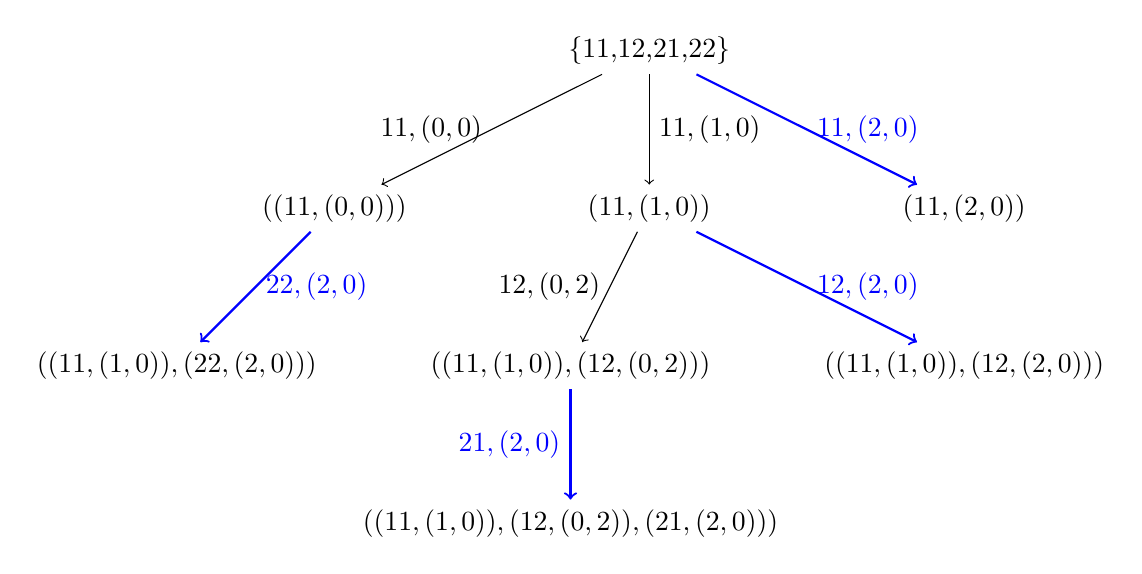
\begin{tikzpicture}
    \node (1) at (0,0) {\{11,12,21,22\}};
    \node (2) at (-4,-2) {$((11,(0,0)))$};
    \draw[->] (1) -- (2) node[pos=0.5, left] {$11,(0,0)$};
    \node (3) at (0,-2) {$(11,(1,0))$};
    \draw[->] (1) -- (3) node[pos=0.5, right] {$11,(1,0)$};
    \node (4) at (4,-2) {$(11,(2,0))$};
    \draw[->, thick, blue] (1) -- (4) node[pos=0.5, right] {$11,(2,0)$};
    \node (5) at (-1,-4) {$((11,(1,0)), (12,(0,2)))$};
    \draw[->] (3) -- (5) node[pos=0.5, left] {$12,(0,2)$};
    \node (6) at (4,-4) {$((11,(1,0)), (12,(2,0)))$};
    \draw[->, thick, blue] (3) -- (6) node[pos=0.5, right] {$12,(2,0)$};
    \node (7) at (-6,-4) {$((11,(1,0)), (22,(2,0)))$};
    \draw[->, thick, blue] (2) -- (7) node[pos=0.5, right] {$22,(2,0)$};
    \node (8) at (-1,-6) {$((11,(1,0)), (12,(0,2)), (21,(2,0)))$};
    \draw[->, thick, blue] (5) -- (8) node[pos=0.5, left] {$21,(2,0)$};
    \end{tikzpicture}
    \caption{Strom algoritmu pro [2,2]-Mastermind}
\label{fig22minmax}
\end{figure}


% možná to není potřeba
%\begin{lemma}[Jednoznačnost hrany]
 %   Nechť $(V, E)$ je graf a $K \in V$ je vrchol. Potom z $K$ vede právě jedna hrana 
%\end{lemma}



% tato definice možná ani není potřeba, protože s ní dále nepracuji
%\begin{definice}[Rozdělení]
 %   Pro $K \subset H_{n,k}$ definujeme rozdělení vzhledem ke kódu $u$ jako množinu potomků $K$, vzhledem ke kódu $u$. $R_{K,u} = \{K_{u,r} \mid r \in S\}$. 
%\end{definice}




% ======================== napsat u obecn0ho algoritmu =====================


\subsubsection{Obecný algoritmus}
Nyní přistoupíme k popisu skupiny deterministických algoritmů řešící hru [n,k]-Mastermind. Algoritmy popisujeme podle funkcí, které pro jakýkoliv stav naleznou další pokus. Nazýváme je, valuace a strategie. 

Pro zjednodušení tyto funkce definujeme pro množiny kandidátů stavů. Pro dva různé stavy, které ale mají shodnou množinu kandidátů je problém nalezení dalšího kódu ekvivalentní. Předpokládáme totiž, že všechny kódy mohou být tajným kódem se stejnou pravděpodobností. Stejné množiny kandidátů pro dva různé stavy lze například dosáhnout prohozením prvků stavu. 

% Ve chvíli, kdy mají nějaké dva stavy stejnou množinu kandidátů, nezáleží na tom, jaké prvky stav obsahuje. Platí, že při následném zvolení stejných pokusů pro oba stavy dosáhneme stejného výsledku. Dojdeme ke stejnému konečnéme stavu.

% Pro dva různé stavy, které ale mají shodnou množinu kandidátů je problém nalezení dalšího kódu ekvivalentní. Předpokládáme totiž, že všechny kódy mohou být tajným kódem se stejnou pravděpodobností. Stejné množiny kandidátů pro dva různé stavy lze například dosáhnout prohozením prvků stavu. 


% K popisu výběru dalšího tahu algoritmy nebudou používat stav hry jako v definici \ref{defstav}. Místo toho vybírají další kód za pomocí množiny kandidátů tohoto stavu. 

% Našim cílem je totiž co nejlépe rozlišit, který kandidát je tajným kódem. Různé stavy které ale mají stejnou množinu kandidátů se v této informaci neliší. Proto výběr dalšího tahu lze vztáhnout pouze na množinu kandidátů aktuálního stavu. 



% U této definice si nejsem jistý, jak to smyslupně definovat. Vazba "která lz e vyjádřit pomocí potomků" se mi moc nelíbí - definovat valuaci a až potom jednokrokové valuace
\begin{definice}[Valuace]
    Nechť $G = (V,E)$ je graf [n,k]-Mastermindu a $K \in V$ je vrchol. Potom valuaci vzhledem k množině $K$ definujeme jako funkci $f_K(u) \colon H_{n,k} \to \mathbb{R}$.
\end{definice}


Valuace bude v algoritmech sloužit pro vyčíslení vhodnosti kódu $u$ jako dalšího pokusu pro stav vyjádřený množinou kandidátů $K\subset H_{n,k}$. Tato hodnota bude obvykle záviset na potomcích $K$ vzhledem ke kódu $u$. Potomci $K$ vzhledem ke kódu $u$ totiž určují možné následující stavy v případě, kdy zvolíme kód $u$ jako další pokus. Valuace nám umožňuje ohodnotit kód podle toho, jak dobré jsou jeho následující stavy. 

\begin{prikl}\label{prjednokrokfce}
    Funkce $f_K$ je příklad valuace, která kódu $u$ přiřadí očekávaný počet kódů potomka $K$ vzhledem ke kódu $u$.
    % jednokrokov8 funkce je taková, která kódu $u$ přiřadí hodnotu, která lze vyjádřit pomocí potomků $K$ vzhledem ke kódu $u$.
    \begin{align*}
        f_K \colon H_{n,k} &\to \mathbb{R} \\
        u &\mapsto \sum_{r\in S}\frac{|K_{u,r}|}{|K|}|K_{u,r}| 
    \end{align*}
    Pro $K = H_{2,2}$ z obrázku \ref{fig22prvnitah} má $f_{K}$ konstantní hodnotu $\frac{3}{2}$.
\end{prikl}
% množinu kandidátů na tajný kód
Obecně valuace nemusí být omezená na následující vrstvu. Mohla by odkazovat na očekávaný počet kódů vrcholu o dvě či více vrstev dál. 

\begin{definice}[Strategie]
    Nechť $\mathcal{F} = \{f_K\colon H_{n,k} \to \mathbb{R} \mid K \subset H_{n,k}\}$ je prostor valuací. Potom strategii definujeme jako zobrazení $F \colon \mathcal{F} \to \mathbb{R}$. 
\end{definice}
% Strategie určitým způsobem slouží k výběru následujícího kódu. 
%Zjednodušeně řečeno slouží k určení, 
Strategie v této práci bude určovat, zda chceme vybírat kódy s vyšší nebo nižší hodnotou valuace.
%Použití bude popsáno níže v popisu algoritmu \ref{alg-default}. 

\begin{prikl}\label{prstrategie}
    Funkce $F$ je strategie, která funkci $f_K \in \mathcal{F} = \{f_K\}$ přiřadí její maximální hodnotu na $H_{n,k}$.
    \[F(f_K) =  \max_{u\in H_{n,k}}\{f_K(u)\}\]
    Strategie je dobře definovaná, protože maximum na konečné množině reálných čísel má vždy jednoznačnou hodnotu.
\end{prikl}

Deterministické algoritmy popisujeme jako algoritmy, které pro následující pokus vybírají kód podle zvolené valuace a strategie. Postup je znázorněn v algoritmu \ref{alg-default}.

% \subsection{Varianty algoritmů}





%Nechť \[P = \left((u_1, r_1), (u_2,r_2), \dots, (u_j,r_j)\right), u_i \in H_{n,k}, r_i \in \N _0 \times \N _0\] jsou tahy s ohodnocením a $K$ je konec cesty $P$ z vrcholu $H_{n,k}$. 

%Potom jednokrokové strategie volí další kód ten, který minimalizuje respektive maximalizuje funkci $f_K$. Pokud je těchto kódů více, zvolí kód, který je zároveň kandidát cesty $P$. Pokud výběr stále není jednoznačný, algoritmus zvolí lexikograficky nejnižší kód. 

\begin{algorithm}[h!]
\begin{algorithmic}[1]  % [1] způsobí, že číslujeme kroky algoritmu
\Function{Solve$[n, k, \mathcal{F}, F]$}{$v$}
    \State $K \gets H_{n,k}$ 
    \State $j \gets 0$
    \State $r_0 \gets (0,0)$
    \While {$r_j \neq (n,0)$} \hfill \mbox{(dokud hra není dohrána)}
        \State $j \gets j + 1$ 
	\State $U \gets \{u \in H_{n,k} \mid f_K(u) = F(f_K)\}$
        \If{$U \cap K \neq \emptyset$}
            \State $u_j \gets$ lexikograficky nejmenší $u \in U \cap K$
	\Else
		\State $u_j \gets$ lexikograficky nejmenší $u \in U$
	\EndIf
        \State $r_j \gets s(u_j, v)$ \hfill \mbox{(ohodnocení pokusu)}
        \State $K \gets K_{u_j,r_j}$
    \EndWhile
    \State \Return $u_j, j$ \hfill \mbox{($u_j$ je tajný kód, $j$ je počet pokusů)}
\EndFunction
\end{algorithmic}
\caption{Algoritmus řešící [n,k]-Mastermind}
\label{alg-default}
\end{algorithm}

Písmenem $K$ značíme množinu kandidátů na tajný kód pro aktuální stav hry (cestu pokusů s ohodnocením). Začínáme s $K = H_{n,k}$. Aktuální číslo pokusu značí $j$, $u_j$ je kód, který algoritmus zvolí jako $j$-tý pokus a $r_j$ je ohodnocení $u_j$ vzhledem k tajnému kódu $v$. Množina $U$ značí kódy, ve kterých valuace $f_K$ nabývá určitou optimální hodnotu danou strategií $F$. Z této množiny algoritmus vybírá další pokus $u_j$. Ve chvíli, kdy existuje kandidát v množině $U$ ($U\cap K \neq \emptyset$), algoritmus zvolí ten, který je lexikograficky nejmenší. Jinak algoritmus volí lexikograficky nejmenší kód z $U$. 

Aby byla strategie $F$ použitelná v algoritmu, musí platit následující podmínka. 
\[\forall K \in V \hspace{5px} \exists u \in H_{n,k} \colon F(f_K) = f_K(u)\]
Pokud by tato podmínka nebyla splněna, mohlo by se stát, že množina $U$ bude prázdná a algoritmus nedokáže zvolit další pokus.

% šlo by napsat pro dvojice funkce f, funkcionál F
%\begin{veta}[Správnost algoritmu \ref{alg-default}]
 %   Algoritmus \ref{alg-default}
%\end{veta}

% \begin{tvrz}[Počet ohodnocení]
% Nechť $n\in \mathbb{N}, k\in \mathbb{N}, k \geq 3$. Potom počet všech možných ohodnocení kódů v $H_{n,k}$ je $\frac{n^2 + 3n}{2}$.
% \end{tvrz}
% \begin{dukaz}
% Pro $b \leq n,\hspace{3px} b \neq n-1$ černých kolíčků existuje $n-b+1$ možností na počet bílých kolíčků podle tvrzení \ref{tvrzohodnoceni}. Pro $b = n-1$ existuje pouze jedno ohodnocení. Součtem přes počet černých kolíčků dostáváme následující počet možností ohodnocení.
%     \[|S| = (n+1) + n + (n-1)  + \dots + 3 + 1 + 1 \]
% Vzorcem pro součet aritmetické řady se dobereme k výsledku.
%     \[|S| = \frac{(n+1)(n+2)}{2} - 1 \]
%     \[|S| = \frac{n^2 + 3n}{2}\]
% \end{dukaz}

% \begin{tvrz}[Časová složitost algoritmu \ref{alg-default}]
%     Uvažujeme případ, kdy $F$ je minimizér/maximizér.
%     Algoritmus \ref{alg-default} má časovou složitost
%     % \[O( k^n O(f_K))\]
%     \[O \left( \sum_{j = 1}^z k^n \cdot m_j \cdot n^2 \cdot \frac{n^2 + 3n}{2}\right)\]
    
% \end{tvrz}
% \begin{dukaz}
%     $k^n$ je počet všech kódů, které musím projít, abych našel ten nejlepší, $m_j$ je maximální počet kandidátů v j-té iteraci, $z$ je maximální počet iterací algoritmu. $\frac{n^2 + 3n}{2}$ je počet všech ohodnocení, $n^2$ je časová složitost ohodnocení.

%     Potřebuji ještě limit na počet iterací $z$, horní odhad na $m_j$ a zjistit složitost nalezení průniku $U$ a $K$.
% \end{dukaz}

